\graphicspath{{content/chapters/1_introduction/figures}}
\chapter{Introduction}
\label{chp:introduction}

Machine learning, commonly referred to as Artificial Intelligence (AI), has seen rapid advancements over the past decade. These advancements have been largely driven by increasing computational power and the availability of large datasets. As a result, machine learning techniques have been integrated into various domains to solve complex problems, including speech processing and noise cancellation. However, this shift toward AI-driven solutions has often lacked thorough evaluation, with justifications for their use and the required computational resources sometimes being unclear.

This project focuses on noise cancellation in audio signals for speech enhancement, a critical area with applications in telecommunications, assistive technologies, and real-time communication systems. Noise is defined as the attenuation or distortion of an original signal caused by external factors, including background sounds in an environment or interference from electronic devices. Background noise can significantly degrade the quality of speech signals, making it difficult to understand or process the conveyed information. Noise can be classified into two categories: stationary and non-stationary \cite{loizou2013speech}.

\begin{itemize}
    \item Stationary noise has a constant power spectral density, meaning its properties remain relatively unchanged over time. An example is white noise, which is random but statistically stable.
    \item Non-stationary noise has a varying power spectral density, meaning its characteristics fluctuate over time. Examples include traffic noise or human chatter, which are unpredictable and more difficult to remove.
\end{itemize}

Two fundamental characteristics of speech are utilized in speech enhancement. Firstly, speech is a non-stationary signal, which helps in distinguishing it from stationary noise. Secondly, speech has a specific frequency range, typically between 300 Hz and 3400 Hz, known as the human voice frequency range. This allows filtering techniques to remove non-speech components while preserving intelligibility.

Noise cancellation is the process of removing unwanted noise from a signal, allowing the original speech to be heard more clearly. Traditional noise cancellation techniques, such as the Wiener filter, estimate and subtract noise from the signal. However, these classical methods often assume stationary noise, which is not always the case in real-world environments. Machine learning-based approaches have emerged as a promising alternative, offering the ability to learn complex patterns and relationships in data without requiring explicit rule-based programming.

\section{Neural Networks for Noise Cancellation}
\label{sec:neural_networks}

Machine learning models, particularly neural networks, have been widely adopted for noise cancellation. Neural networks, inspired by biological neurons in the human brain, are composed of layers of interconnected processing units known as \textit{neurons}. Each artificial neuron receives multiple inputs, performs a weighted summation, applies a bias, and passes the result through an activation function to produce its output.

This structure draws direct inspiration from the way biological neurons function—where dendrites receive signals, the cell body processes them, and the axon transmits the signal to the next neuron. Figure~\ref{fig:neuron_vs_ann} illustrates this analogy.

\begin{figure}[H]
    \centering
    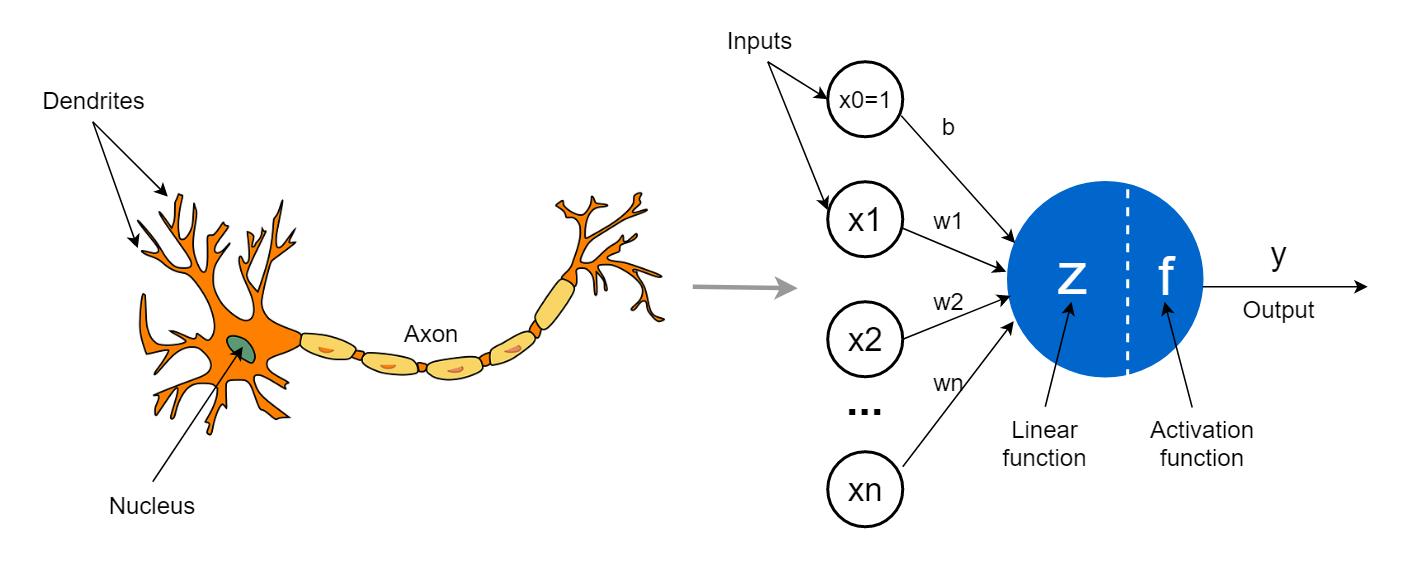
\includegraphics[width=0.75\textwidth]{neuron_vs_ann.png}
    \caption{Biological neuron vs. Artificial neuron structure.\cite{ghosh2020perceptron}}
    \label{fig:neuron_vs_ann}
\end{figure}

A typical neural network for noise cancellation consists of the following components:
\begin{itemize}
    \item \textbf{Input layer:} Receives the noisy speech signal (e.g., a time-domain waveform or its spectrogram).
    \item \textbf{Hidden layers:} Perform nonlinear transformations to extract key features and patterns from the input. These layers may include convolutional, recurrent, or fully connected neurons depending on the network architecture.
    \item \textbf{Output layer:} Produces the denoised speech signal by mapping the learned features back to the clean signal domain.
\end{itemize}

The network is trained using pairs of clean and noisy audio samples. It gradually learns to reduce the difference between its predicted output and the actual clean signal. Once trained, the model can take in new noisy speech and output a cleaner version. This learning-based approach allows neural networks to adapt to complex noise patterns, often performing better than traditional signal processing methods in real-world situations.

\section{Project Goals and Implementation}

The primary goal of the project is to explore both classical and machine learning-based approaches to noise cancellation, evaluating their effectiveness and feasibility in real-world applications. The project will not only examine established noise reduction techniques but also develop a machine learning-based model, comparing its performance against classical methods.

The approach involves designing and implementing a noise cancellation system that operates under the assumption of a single-speaker scenario in a noisy background environment, where the system must remove both stationary and non-stationary noise without access to a clean reference signal. Unlike established pre-trained models that required extensive datasets and resources, the model developed in this project will not be pre-trained, allowing for a demonstration of the ease of developing and training in practical settings. However, during evaluation and benchmarking, pre-trained models will be used for comparison to assess their effectiveness against the proposed approach.

The project will be implemented in Python using a modular and reproducible structure, ensuring that the framework can be extended or modified for further improvements. The project is structured into three core phases: training, denoising, and deployment
\begin{itemize}
    \item Training phase: The most computationally intensive stage, where a sourced dataset of clean and noisy speech samples will be formatted and fed into the model to learn respective mapping.
    \item Denoising phase: Involves loading the trained model and applying it to a noisy speech signal to generate a cleaned output. Here evalution metrics will also be producable to assess the performance of one methodology against another.
    \item Deployment phase: The final phase involves simulating a real-world application scenario. After training ad justification through performance evaluation, the model will be embedded into a real-time application. This will essentially be a remake of the denoising phase, but with the model integrated into a board that will take real time input sequence from a microphone and save the denoised output. The label for real-time will be indicated through evaluated inference time calculated during the denoising phase.
\end{itemize}


\section{Overview of the Contents of the Report}